% !TEX root = ../thesis-example.tex
%
\chapter{Summary, Conclusions \& Future Prospects}
\label{Chap:Conclusions}
\cleanchapterquote{From the point of ignition \\
To the final drive \\
The point of the journey \\
Is not to arrive \\
Anything can happen}{Neal Peart}{Prime Mover, Rush}


\section{Advantages of an Analysis in Harmonic Space}
\label{sec:conclusion:Harmonic}
One of the main objectives of this work was to demonstrate how powerful a spherical harmonics analysis of the large scale structure of galaxies is in order to constrain cosmological models and parameters. For a spectroscopic survey such as BOSS, taking the route of a spherical harmonics analysis can be counter-intuitive. Spectroscopic samples have outstanding redshift measurements, allowing for a standard 3D analysis of clustering to be performed with extreme accuracy. This is mostly since no systematic limiting factors from the imprecision of photometric redshift determination are present. From a phenomenological point-of-view, there are no advantages in performing an analysis in harmonic space since it seems like radial information is mostly lost due to projection effects. One would naturally argue to perform the analysis in 3D, i. e. using the 3D power spectrum $P(k)$, instead. 

\qquad However, dealing with proper data is quite different from what we conceptualise in the `pre-survey' years and Fisher forecasts. To perform standard 3D analysis, one needs to first choose a fiducial cosmology to perform a change of coordinates from redshift space to co-moving space. This approach has the potential to bias cosmological results on its own and few studies in the literature actually analyse the impact of choosing an incorrect fiducial cosmology. It is expected that, if not too far from the true cosmology, the bias cause by these assumptions should be sub-dominant to the statistical precision one has in the overall cosmological analysis. Here, I outline the first practical advantage of an analysis in harmonic space: as the analysis is performed in projected space, there is no need to change coordinates, the whole analysis is performed in redshift space -- what is actually being measured in the spectrographs of our telescopes (for spectroscopic surveys).

\qquad In this work, I have shown that it is possible to recover very powerful and competitive cosmological constraints from spectroscopy alone with a 2+1D analysis -- as good as the constraints from doing a 3D analysis. The precision of spectroscopic redshifts allows for very fine radial binning, probing the evolution of structure in more detail. The `effective redshift' approximation impacts 3D analyses, complicating the proper treatment of `light-cone' effects. By contrast, this is not a problem with $C_{\ell}$s as one is dealing with data in redshift space using a fine binning. Once more, as I am using data in redshift space, no transformation to comoving coordinates is necessary, and hence no fiducial cosmology is required. I argue that it is much simpler in Fourier space than in real space to correct certain types of systematic errors and to perform scale cuts to deal with non-linearities; the arguments here are similar to the ones used to compare $P(k)$ and $\xi(r)$.

\qquad As outlined in Chapter \ref{Chap:Neutrinos}, the angular power spectra of galaxies have also a different dependency and sensitivity to neutrino related parameters. More specifically, the sum of neutrinos masses, \NM, seems more sensitive in harmonic space -- possibly due to the projection of the line-of-sight information. Although, it is clear that when working in 2+1D, an improper care of the galaxy shot-noise could lead to under-estimated values of the upper bound of \NM.

\qquad In conclusion, I would like to point out that the biggest advantage of performing this 2+1D tomographic analysis in harmonic space is the practicality of combining spectroscopic and photometric probes, which include also cosmic shear, as the latter also ``lives" in a 2+1D space. Using the method proposed by \cite{2016McLeod} the spectroscopic sample has the potential of ``fixing" the photometric redshift limitations when probing the photometric clustering redshift distribution together with the cosmological parameters.


\section{$\Lambda$CDM: Final days?}
\label{sec:conclusion:sec2}
As I finish this work, the last round of big survey's results is out (for a while now) and it seems like none of us broke the standard model of cosmology (yet!). With the exception of a few parameters like $H_0$ \citep{2018HubbleMortsell, Riess2018} and $\sigma_8$ \citep{2015MacCrann}, it seems like the standard model of cosmology is well agreed between surveys -- both from late or early times. The before-mentioned discrepancies and tensions between early cosmology probes like Planck and late cosmology galaxy surveys such as KiDS and CHFTLens could hint that new physics is on the horizon. If there's differential growth of structure, or some redshift dependency and evolution on some parameter, we could be missing out information by performing the standard 3D analysis in a box. It could be the case that a tomographic analysis could hint into solving this mysteries. It could also be the case that we will soon find that such tensions arise from unknown systematic effects.

\qquad Meanwhile, when probing the $\Lambda$CDM parameters from the BOSS-$C_{\ell}$s dataset and comparing the infered cosmological parameters from those obtained by an analysis of the Planck data, no relevant tensions are observed for $H_0$ -- mostly due to the BOSS dataset not having sufficient constraining power on its own to narrow the Hubble Constant. However, in terms of the clustering amplitude, a significant difference was found with $S_8^{\text{BOSS}} = 0.715^{+0.072}_{-0.064}$ while the CMB probe exhibits a $S_8^{\text{Planck}} = 0.850^{+0.023}_{-0.021}$. This indicates a tension that is worth further investigation as figure \ref{fig:Om_S8_LCDM} demonstrates agreement with shear measurements from KiDS \citep{2017MNRAS.465.1454H}.

\qquad From a different perspective, hopes for our first step towards breaking free of $\Lambda$CDM could also come from a measurement of the equation-of-state of dark energy which implies something different than an accelerated expansion caused by the cosmological constant; i.e. $w_0 \neq -1$. Nonetheless, as the precision $w_0$'s measurements reaches a percent level, hopes of finding a way out of $\Lambda$CDM via $w_0$ are starting to seem unlikely. Even so, in this work I have demonstrated that combining measurements from BOSS DR12 in harmonic space with Planck and JLA one can obtain extremely competitive precision for this parameter with $w_0 = -0.993^{+0.046}_{-0.043}$ -- one of the most precise measurements in the literature. Once more,  this measurement of the equation-of-state of dark energy seems to strongly suggest a scenario where the expansion is caused by the cosmological constant. On a different note, I would like to point out once more a very small tension between BOSS and Planck when it comes to the amplitude of clustering: $S_8^{\text{BOSS}} = 0.726_{-0.061}^{+0.072}$ while $S_8^{\text{Planck}} = 0.811_{-0.037}^{+0.034}$.

\qquad In conclusion, it is hard to predict whether or not we will have 20 more years of $\Lambda$CDM or if we will be able to break it in the next following years. One thing is for sure, combining cosmological probes will be key if we want to move away from the current paradigm; a harmonic space analysis being an extremely versatile approach to move down this route.


\section{Neutrinos: Beyond the Sum}
\label{sec:conclusion:sec2}
As the scenario of a new paradigm shift in cosmology seems to be in the horizon for the past 20 years, our attention shifts towards other problems in which cosmology can give complementary knowledge. This could also obtain hints on what could be going wrong with our current strategy of breaking the current standard model. Like cosmology, neutrino physics also had a major breakthrough in the past 20 years, causing serious damage to the Standard Model of Particle Physics. The fact that neutrinos have mass and oscillate between their three leptionian flavours was a first step beyond the Standard Model. Yet, particle physics experiments can say little about the absolute mass scale of neutrinos (\NM) or even less about the mass of the lightest neutrino species without making any strong model assumptions and inferences from null results \citep{2016KamLANDMajorana}.

\qquad In Chapter \ref{Chap:Neutrinos}, I have demonstrated that cosmological measurements from combined probes such as BOSS, Planck, Pantheon and some BBN prediction can be combined with neutrino oscillation constraints from global fits to obtain information on neutrino parameters using an exact approach. The usual approach taken by cosmological surveys is to either ignore or model neutrino masses using approximations for \NM. I have demonstrated here that such route of approximations can lead to dangerous discrepancies as they are model dependent given the current constraining power. 

\qquad In the meantime, using exact models -- which take into account constraints for the square mass splittings $\Delta m_{21}^2$ and $|\Delta m_{31}^2|$ -- yields robust constraints on the upper bound of \NM{} while also obtaining a model-free upper bound on the mass of the lightest neutrino, $m_0^{\nu}$. Using this approach, I obtained an upper bound as low as $m_0^{\nu} > 0.086\, eV$ with a combination of cosmology and oscillation experiments. As far as the literature goes, this is one of the first times, if not the first, that an upper bound on this quantity is set without an assumption about the neutrino's mass mechanism. This opens a whole new door for cosmological experiments to liaise with particle physics in order to narrow down the neutrino mass parameter space from a different perspective. This is shown in Figure \ref{fig:Major} for the case of searching for Majorana neutrinos in neutrino-less double-$\beta$ decay ($0\nu\beta\beta$) experiments \citep{2016DoubleBetaReview}. 

\begin{figure}
\begin{center}
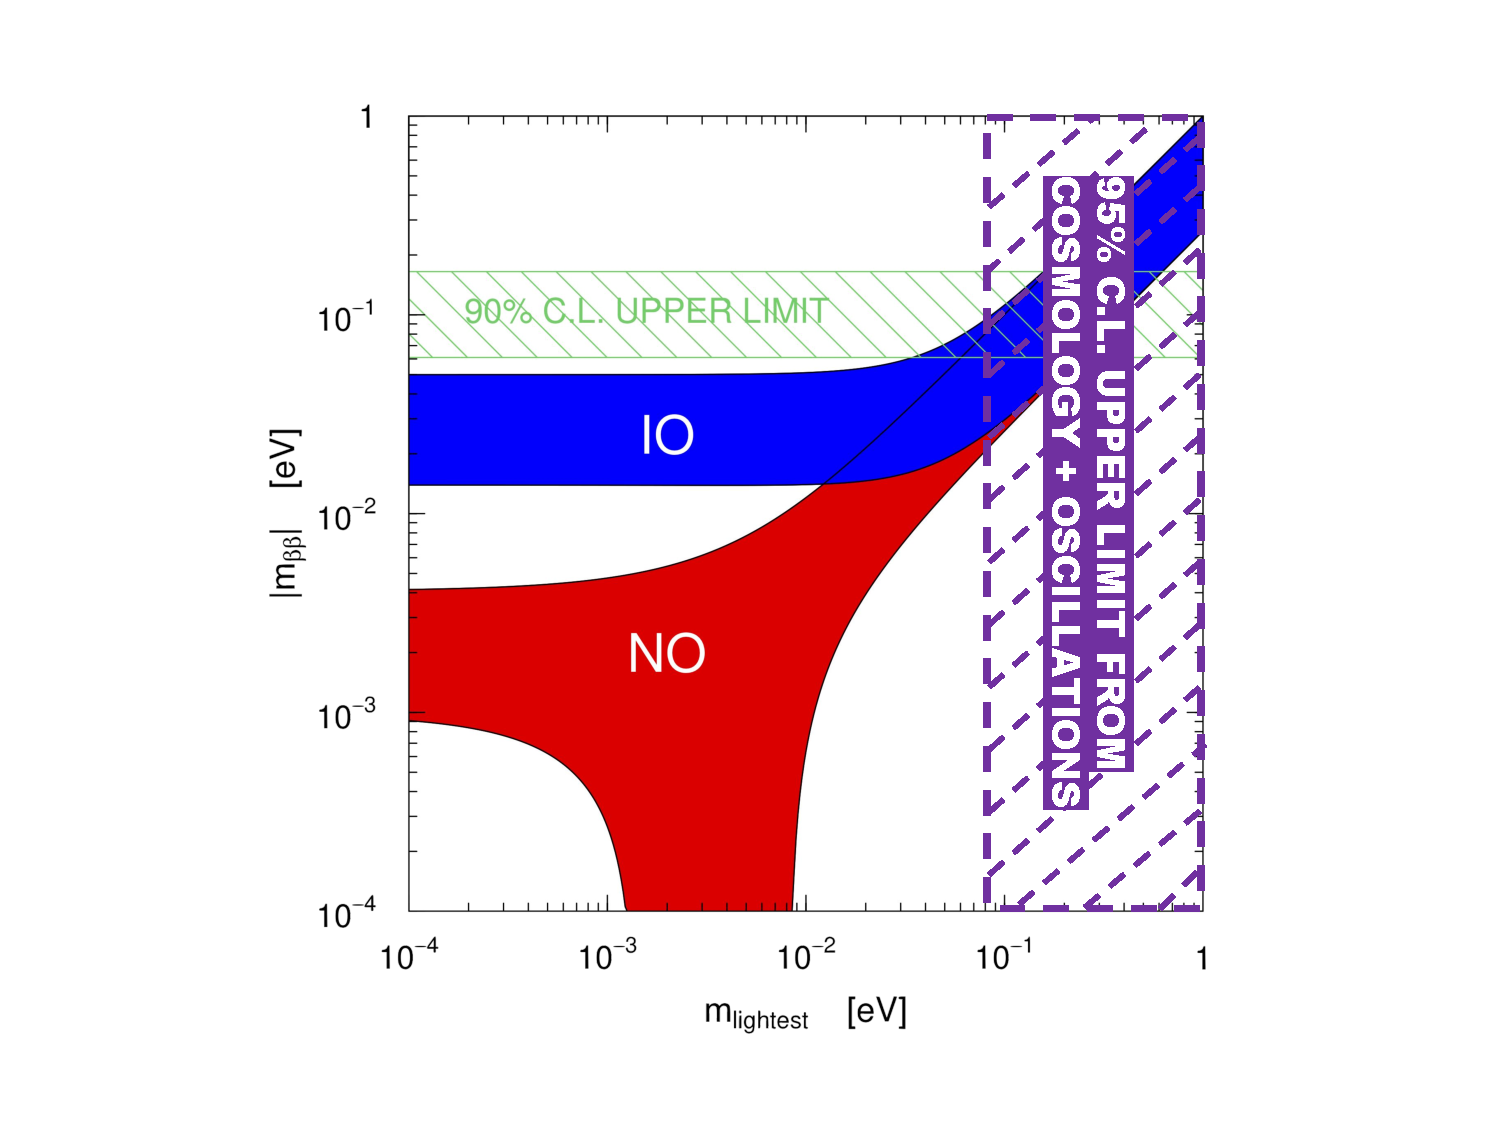
\includegraphics[scale=0.60]{Intro-FIGS/doublebeta.pdf}
\caption[The effective Majorana neutrino mass, $|m_{\beta\beta}|$, as a function of the lightest neutrino species mass.]{The effective Majorana neutrino mass, $|m_{\beta\beta}|$, as a function of the lightest neutrino species mass, $m_{\text{lightest}}$ -- previously referred to as $m_0^{\nu}$. The red (blue) shaded regions are the 99.7\% C.I. for the normal (inverted) ordering (or hierarchy). The green shaded region shows the 90\% C.I. upper bounds obtained with null results from the KamLAND-Zen Experiment searching for Majorana neutrinos \citep{2016KamLANDMajorana}. The purple shaded region shows the 95\% C.I. upper bound on $m_{0}^{\nu}$, the main result from Chapter \ref{Chap:Neutrinos}. This diagram demonstrate the advantages of performing a neutrino analysis using an exact model while combining cosmological probes with oscillation experiments. The purple shaded region is independent of neutrinos being Majorana, Dirac or variations. Image Credit: Adapted from \cite{2018MassOrdering}}
\label{fig:Major}
\end{center}
\end{figure}

\qquad Following this approach, cosmologists and particle physicists can work together in the search to fix the Standard Model of Particle Physics while moving towards breaking the Standard Model of Cosmology, $\Lambda$CDM. It is possible that current analysis in cosmology, in which $\sum m_{\nu} \lesssim 0.14\, eV$ \cite{2015LyAlpha-Deg,2016Cuesta-Deg} could have achieved a much tighter upper bound on $m_0^{\nu}$ have they decided to go down the same route and combine cosmology with neutrino oscillation constraints. Even though, results are such that a cosmological neutrino detection seems to be in the near future, possibly with the cross-correlations between spectroscopic and photometric surveys -- in order to achieve both a high volume of galaxies and high redshift estimation precision.
%\Blindtext[3][2]

\section{Towards primordial non-Gaussianities: Bayesian-$C_{\ell}$ estimator and $f_{nl}$}

\section{Future Work} 
\subsection{Preparing for Euclid, DESI, and more}
\label{sec:conclusion:future}
With increasingly large future photometric and spectroscopic surveys such as LSST \citep{2012arXiv1211.0310L}, DESI \citep{2016-DESI}, J-PAS \citep{JPAS}, and Euclid \citep{2011EuclidRedPaper}, the future of precision cosmology lies in the ability to combine datasets from across the entire electromagnetic spectrum. The angular power spectrum approach offers a unified framework for coherently combining different datasets in order to obtain maximal information from each \citep{JoachimiBridle2010,Kirk2015,2016McLeod}. I believe that the approach used in this work, in which cosmological information is extracted from the projected distribution of the galaxies in a spectroscopic survey, is a useful step towards achieving this unified framework. I further claim that this approach leads to a better understanding of the evolution of structure in the Universe as it provides more information on the redshift evolution of galaxy bias.

\qquad For future redshift surveys such as DESI and J-PAS, which will obtain unprecedented redshift precision in their measurements while also probing a much larger volume in the sky, this methodology would have many advantages, previously pointed out in Section \ref{sec:conclusion:Harmonic}. With such large volume, it is possible that DESI alone could have a breakthrough in neutrino masses, although further investigation is necessary. Performing a neutrino forecast with $C_{\ell}$s is one of my `near-future objectives'.

\qquad In the case of Euclid and LSST, the key to obtain state-of-the-art cosmological measurements from these surveys will rely on the ability to cross-correlate them to counter-balance their limitations with their advantages. Euclid will have low-resolution spectroscopy with extremely good photometry (since it is a space probe); however, it will only use a few bands in visual and near-infrared. In the other hand, LSST will perform a state-of-the-art ground-based photometric survey in five different bands, mostly in the southern sky. Many of the possible synergies between both surveys have been recently discussed by \cite{2017EuclidLSST}, with focus on using Euclid's spectroscopy to calibrate LSST's photometric redshift. As a future research interest, I belive that taking an approach as the one in \cite{2016McLeod} could maximise advantages as it probes the photometric redshift distribution and cosmological parameters using the cross-angular power spectra between the photometric and the spectroscopic samples. 

\qquad On the context of Euclid, I will be working during the following year as an Euclid Post-Doctoral Research Associate at University College London with the purpose of extending the pipelines I have developed for the BOSS study to weak lensing measurements for power spectra estimation of shear and convergence fields. I will work on development, validation and verification of the weak lensing pseudo-$C_{\ell}$ pipelines, including also covariance matrix estimation for these measurements. Further development on the Bayesian-$C_{\ell}$ estimator outlined in Section \ref{Sec:BPL} will also aid in benchmarking the pipelines. This will allow me to extend the horizons and prepare the grounds from when future observations from Euclid are available. These pipelines will also be tested with Euclid flagship simulations and, possibly, with public photometric data from the KiDS Collaboration \citep{2017KiDS-DR3}.

\subsection{Neutrino Masses \& Non-Gaussianities}
Future surveys such as Euclid, DESI, and LSST will have the potential to solve key cosmological questions. Two of them, regarding neutrino properties and non-Gaussianities in the early Universe, are my main focus of interest. Due to their large survey volumes, these cosmological instruments are ideal to set extremely accurate and precise constraints for neutrino parameters such as $\sum m_{\nu}$, the hierarchy, and $m_{0}^{\nu}$, together with early universe parameters such as $f_{nl}$. DESI, Euclid, and LSST have a great potential to obtain galaxy samples beyond just the usual red and blue samples. Cross-correlations between these surveys could solve photometric redshift estimation issues. Photometric surveys like Euclid, LSST, and KiDS will additionally obtain unprecedentedly accurate shape measurements for weak lensing measurements. My future research will be focused on obtaining not only precise cosmological measurements, but also accurate cosmological measurements. One of my key objectives is to deal with effects that bias our cosmological conclusions: both methodological (e.g. redshift distribution estimation, fingers-of-god, intrinsic alignments) and observational (e. g. seeing, psf, extinction). Here, once more, I argue that the use of angular power spectra as a unified framework allows for optimal control of such systematic issues.

\qquad In most cases, methodological systematics can be modelled into a concise Bayesian framework and treated as nuisance parameters while probing the cosmological parameters of interest. Effects like extra Poissonian shot-noise can easily mimic lower neutrino masses as these also tend to increase power in all scales. This can be avoided by considering extra shot-noise as a nuisance parameter in the cosmological analysis. However, this approach is only possible when the modelling of phenomena is an option. For cases where unknown or observational systematics are at play, methods like mode-projection can be used within the $C_{\ell}$ framework to deal with systematic effects which affect specific scales \cite{Boris2013}. For non-Gaussianities studies, most of the information about $f_{nl}$ is contained in large scales, meaning that multiple galaxy tracers and quasar samples are necessary to beat the effects of cosmic variance.

\qquad Throughout this work, I have acquired the skills to analyse cosmological data sets, from galaxy catalogues to cosmological parameters estimation, which include: sample selection, map and mask creation, generation and validation of simulations for pipeline verification and covariance matrix estimation, systematic error analysis and mitigation using cross-correlations, galaxy clustering analysis using a Pseudo and a Bayesian $C_{\ell}$ approaches. In \cite{2018LoureiroBOSS} (also presented in Chapters \ref{Chap:BOSS} and \ref{Chap:BOSS-Cosmo}), I simultaneously constrained methodological effect's parameters with cosmological parameters in a concise Bayesian framework and with minimal loss of precision. In \cite{2018LoureiroNeutrinos} (also presented in Chapter \ref{Chap:Neutrinos}), I obtained robust constraints for the upper bound of $\sum m_{\nu}$ and the lightest neutrino mass using a combination of cosmological probes and particle physics constraints. I showed that physically motivated models yield robust results compared to the commonly used cosmological approximations. In \cite{2016AbramoSeccoLoureiro}, I worked with developing and testing a $P(k)$ estimator for multi-tracer analysis in 3D. However, with the experience I have acquired in the last few years, implementing a multi-tracer analysis in harmonic space is much simpler. The tomographic nature of this type of analysis probes larger scales in a much simpler way than in the standard 3D method.

\qquad The applications of the these spherical harmonic analysis techniques -- and the inclusion of mode-projection techniques -- to Euclid, LSST, DESI, KiDS and a combination of these are a natural extension of my current research. Using these techniques, In the near future, I will further constrain neutrino parameters such as $\sum m_{\nu}$, the hierarchy, and $m_{0}^{\nu}$ with unprecedented accuracy and precision. Cross-correlations between these photometric and spectroscopic samples will overcome the potential redshift distribution uncertainty for the photometric samples -- a limiting factor in most photometric surveys \cite{2016McLeod}. I will work towards producing realistic neutrino forecasts as I prepare the frameworks to deal with both methodological and observational effects once data is available. In terms of primordial non-Gaussianities, I will use tomographic redshift bins to simultaneously probe the scale dependent bias and other cosmological parameters; taking into account the correlations between them, which is key for obtaining reliable cosmological measurements. Using this framework I will mitigate effects such as redshift distribution uncertainties, redshift space distortions, and fingers-of-god. I will implement extensions to the work I have developed for different models of scale dependent bias and dependencies on primordial non-Gaussianity models. I will achieve this by performing a multi-tracer analysis with cross-correlations between LSS, weak lensing probes and current CMB data. I will test these methods with state-of-the-art simulations for future surveys, and also apply them to current data from SDSS, KiDS, eBOSS, and Planck using the systematic errors mitigation techniques mentioned above. 

\section{Final Summary}
In summary, throughout this work I have laid out all steps to perform a full cosmological analysis of large scale structure galaxy samples in harmonic space and how to use cosmological measurements, together with particle physics experiments, to set constraints on the lightest neutrino mass. I started from the galaxy catalogues and observational masks; I performed clustering measurements, covariance matrix estimation, systematic analysis, and consistency checks; I demonstrated how powerful such approach is by constraining vanilla $\Lambda$CDM and $w$CDM models and finished by demonstrating that using such approach, cosmological observations can be combined with particle physics constraints from neutrino oscillation experiments to obtain one of the first upper bounds on the mass of the lightest neutrino species.

\vspace*{\fill}
\cleanchapterquote{Eu agradeço ao povo brasileiro \\
Norte, Centro, Sul inteiro \\
Onde reinou o baião}{Caetano Veloso}{You don't know me}